

%\section{Proof of Concept for Future Research}
\section{Needs for Tool Support to Support Third-Party Software Library Adoption (RQ2)}
We discovered from the barriers developers face in the library adoption process that besides organizational limitations, developers are also impacted by the lack of selection tools. Hence, during our qualitative study, we also came up with potential solution proposals for selection tools and evaluated the usability of those solutions. We also collected feedback from our interviewees through an additional survey on the latest technology tools like ChatGPT and its potential usage in library selection.

In this section, we will explore two potential library selection tools along with their motivation and industry evaluation. We shall also present a default priority score of selection factors that can be used by any library selection tool.

\subsection{Library Selection using a Conceptual Tool}
We conceptualized a library selection tool combining the findings of our qualitative research and marketing theories.
\subsubsection{Concept Development from Marketing Model on Buyer Behavior}
During our interview analysis, we found that our \model\space is similar to consumer and business buyer behavior models and decision process of marketing theories \cite{kotler2014principles}. The exact comparison of the models and the buying decision and adoption processes are shown in Figure \ref{fig:model-comparison} and in Figure \ref{fig:process-comparison}.

\begin{figure*}
    \centering
    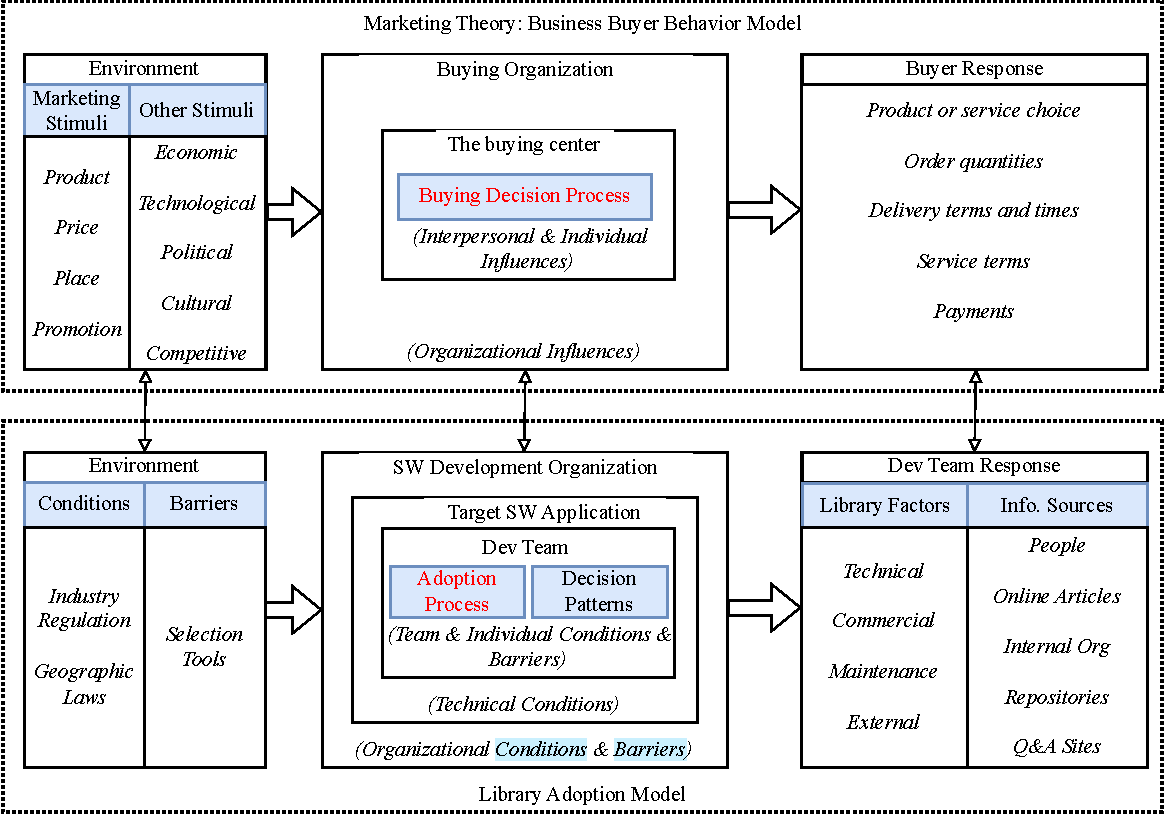
\includegraphics[scale=0.8]{images/Buyer-behavior-models-comparison.pdf}
    \caption{Similarity between \model\space and business buyer behavior model redrawn verbatim from marketing theories \cite{kotler2014principles}. The similar blocks between the two models are mapped using the arrow. While the major building blocks of the two models are identical, in addition to the marketing model, we found \principle\space, challenges, and technical conditions in the \model.}
    \label{fig:model-comparison}
\end{figure*}

\begin{figure*}
    \centering
    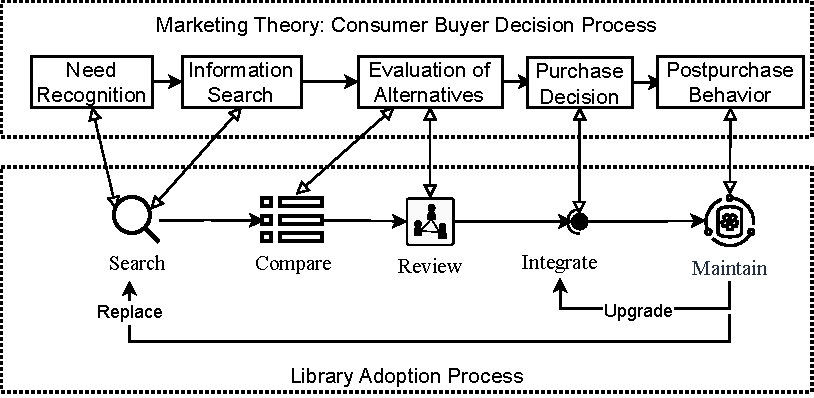
\includegraphics[scale=.8]{images/Decision-adoption-process-comparison.pdf}
    \caption{Similarity between consumer buyer decision process redrawn verbatim from marketing theories \cite{kotler2014principles} and library adoption process. The similar steps between the two processes are mapped using the arrow.}
    \label{fig:process-comparison}
\end{figure*}

The adoption conditions in our model match with business/organization buyer behavior conditions. The two models are also similar in terms of actors. However, unlike the business buying behavior model which has supplier search, selection, and performance review for the traditional procurement process, the library adoption process is simpler and closely relates with the consumer buying behavior. The consumer buying process has need recognition, information search, alternative evaluation, purchase decision, and post-purchase behavior. In our \model, we have split the purchase decision to \code{review} (where most decision is taken) and \code{integrate} steps and merged \code{problem identification} under \code{search} step. Since \model\space resembles the consumer buyer behavior process, it also opens up opportunities to utilize further marketing models in the library adoption process. For example, if Fishbein Multiattribute Model \cite{fishbein1967attitude} can be applied to the consumer model, it can also be applied to the library adoption model. In Multiattribute Model, two products can be compared based on certain factors (f). Each factor has an associated weight (w). The consumer assumes a certain score (s) for each product based on every factor and calculates a net score (NS) by computing the weighted average of the factor scores (s) and weights (w). For example, if there are n factors for a product (P), then the net score (NS) according to Multiattribute Model is calculated using the equation \ref{eq:multiattribute-model}.
\begin{equation}
    NS_p = \frac{\sum_{i=1}^{i=n}w_i*s_i}{\sum_{i=1}^{i=n}w_i}
    \label{eq:multiattribute-model}
\end{equation}


Hence, if we can propose a tool based on the weighted average of different library selection factors, developers might be able to find it useful for decision making as our participants also noted. Based on this assumption and marketing theories, we move forward with a library comparison tool. 

\subsubsection{Mock Up of a Library Selection Tool}
\label{sec:mock-up}
As we proceeded with the interviews, the library selection factors and process were maturing early in the research phase (after around the 8th interview). We have frequently heard from the interviewees about the variation of priorities of different library selection factors. Depending on the particular situation of the target application, under diverse organizational cultures and team dynamics, developers often change their priorities. We decided to apply our analyzed findings to see if that would help developers.

Following our findings, we started discussing with the interview practitioners an applicable tool that can be used in the industry. We experimented with a dynamic weight mechanism for each decision-making factor. Developers can customize such factors based on their situation and by calculating a weighted average of all necessary factors of alternative libraries, developers can finally come to a more structured method of their library comparison. 

After the 8th interview, we designed a mock user interface (UI) for comparative analysis with the weight of factors and demonstrated the interface to the subsequent interviewees. A sample comparison between two Java libraries Jackson and Gson for JSON data processing is presented from the mock UI in Figure \ref{fig:ui-library-comparison}.
\begin{figure*}
    \centering
    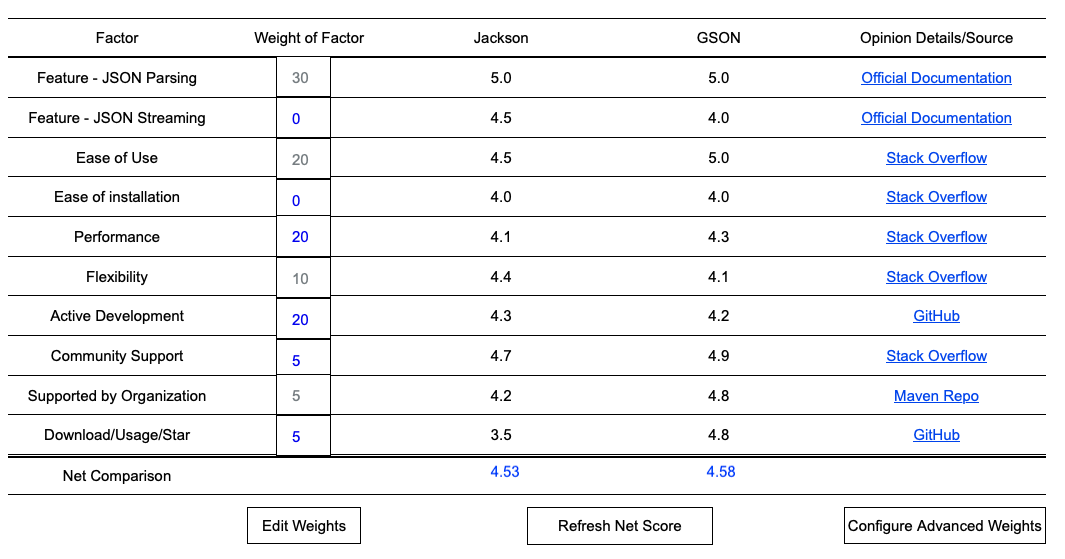
\includegraphics[scale=0.4]{images/mock-ui-library-comparison-2.png}
    \caption{Mock up of a sample comparative analysis of two libraries.
    Some default weights can be provided at the beginning and developers can be able to update the weights (blue-colored weight means the weight is modified by the developer). The score under each library is provided for each aspect and should be ideally calculated by mining the source shown in the Opinion Details/Source column.}
    \label{fig:ui-library-comparison}
\end{figure*}

The first column in the comparison chart contains a few decision-making functional and technical factors. The second column Weight of Factors takes input weights from the developers for their particular situation. The scores under two libraries' columns (Jackson and Gson) contain an aggregated score from the data analysis on respective factors. For example, to measure the score of ease of use, we would mine developers' sentiment in Stack Overflow regarding the specific libraries and come up with a score out of five based on the positive or negative comments shared there. Some scores can be populated using quantitative data collection such as extracting Star (favorite) or measuring recent development activity from GitHub. We would also share the reference of the actual sources from which we are measuring this score in the last column Opinion Details/Source. The final outcome of the analysis is the net comparison of the weighted average score calculated using the Multiattribute Model equation \ref{eq:multiattribute-model}, referred to earlier for each of the two libraries shown in the bottom summary line in blue color. 



\subsubsection{Evaluation of the Library Selection Tool}
All the interviewees highly appreciated such a structured approach to a highly subjective decision that they need to take on a regular basis. Interviewees found the side-by-side numerical comparison to be helpful and suggested a few improvements. For example, instead of providing numerical weight factors, some of them suggested keeping the weights in the backend and in the interface just letting the user choose and rank up and down the priority of the aspects. Some of them also asked for the possibility of manual curation to add new libraries or relevant comments. Most of them requested some way for drilling down to see how the scores are created with some actual references:
\qi{I think that the idea of comparing libraries is quite interesting. If I can click into the underlying sources, then that's pretty interesting for me. I would really value somehow seeing some samples.
... It might be interesting as well to consider whether there is a way to combine both the automated approach plus curated one. People can easily add if there is another library they think should be added.}{P18}

The weighted average decision-making process that was inspired by Fishbein Multiattribute Model \cite{fishbein1967attitude} from the consumer model resonated with most of the participants:
\qi{Yeah. I really like the concept and I'm glad you showed this as an example because I myself have done these sorts of comparisons between Gson and Jackson multiple times. And I really like the variable weight feature because that makes sure that you can focus on what is important for your use case.}{P13}

We assume that future research work can implement the large-scale online review mining and summarize the performance of libraries following this proposed comparative analysis to provide a helpful tool to the developers.

\subsection{Library Selection using ChatGPT and BARD}
\subsubsection{Motivation for Using ChatGPT and BARD}
We conducted the majority of our interviews during the second half of 2022 and a few interviewees mentioned about the usage of ChatGPT\footnote{\url{https://openai.com/blog/chatgpt}} for library-related information collection sources. However, during the analysis part in the first half of 2023, ChatGPT became the fastest-growing consumer application in history \footnote{\url{https://www.reuters.com/technology/chatgpt-sets-record-fastest-growing-user-base-analyst-note-2023-02-01/}}. In February 2023, Google also released similar generative AI-based conversational chatbot BARD \footnote{\url{https://blog.google/technology/ai/bard-google-ai-search-updates/}}. 
If these chatbots can reliably provide library comparison, then this could be a significant support for developers. 
Hence, for the sake of the completeness of study, we wanted to assess the potential usage of ChatGPT and BARD in the library selection process. 

\subsubsection{Experiment with ChatGPT and BARD for Library Selection}
To generate a similar comparison of our proposed mock UI, we provided the following prompt to both ChatGPT and BARD: 
\begin{quote}
  \textit{  Compare Jackson and GSON libraries based on the following aspects (JSON Parsing, Ease of use, Performance, Flexibility, Active Development, Community Support, Supported by Org, Download) in a comparison table. Rate each aspect out of 5 for each library.} 
\end{quote}
Both chatbots provided a tabular comparison against the above prompt as shown in Figure \ref{fig:chatbot-comparison}
\begin{figure*}
    \centering
    \begin{subfigure}{.48\textwidth}
    \centering
        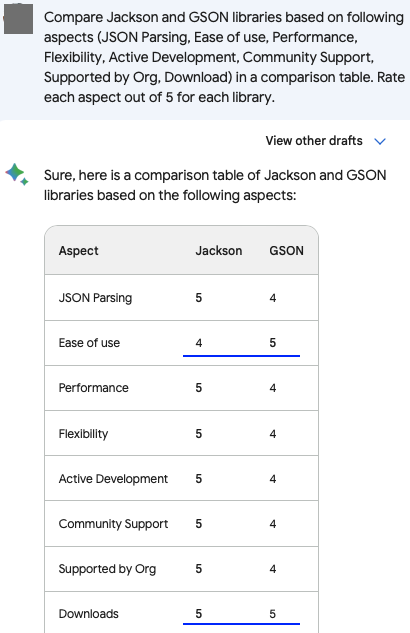
\includegraphics[scale=.5]{images/BARD-Response.png}
        \caption{Response from BARD}
    \label{fig:bard-table}
    \end{subfigure}
    \begin{subfigure}{.48\textwidth}
    \centering
        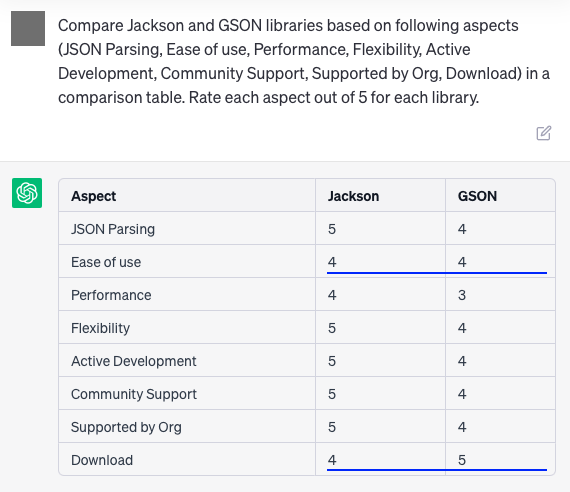
\includegraphics[scale=.4]{images/ChatGPT-Response.png}
        \caption{Response from ChatGPT}
    \label{fig:chatgpt-table}
    \end{subfigure}
    \caption{Response of BARD and ChatGPT for comparing two libraries along with scores.}
    \label{fig:chatbot-comparison}
\end{figure*}

Apparently, both of the models preferred Jackson over GSON. The response shows inconsistent scores between the two models for two different aspects - \code{ease of use} and \code{download count} (\code{download count} is used as an indicator of \code{popularity} factor). BARD gave Jackson (4) a lower score than GSON (5) for \code{ease of use} whereas ChatGPT scored both the same (4). ChatGPT gave Jackson (4) a lower score than GSON (5) for \code{download count} whereas Jackson scored both same (5). Other than these two contradictions, seemingly the chatbot responses were reasonable. Still, we wanted to check the reliability of the response using another small test.

Since in order to identify the score of \code{ease of use} for the two libraries, we shall have to collect reviews online or from other practitioners, we rather chose the \code{download count} which can have a more objective data point. We then asked both chatbots the following prompt: \textit{What is the artifact usage count of Jackson and GSON libraries?}

ChatGPT could not provide any numeric answer because its cutoff date is before September 2021. So we chose BING chat\footnote{\url{https://www.microsoft.com/en-us/edge/features/bing-chat}} to represent ChatGPT since BING chat also uses the same underlying GPT model as ChatGPT. The response from BING chat and BARD are shown in Figure \ref{fig:chatbot-comparison-download}. As we can see, BARD reported the libraries to be used in more than 1.2 million artifacts whereas BING chat referred to an online article and reported that these libraries are downloaded only 14 times (GSON) and 1 time (Jackson). In really, we checked the Maven central repository and found that both of the libraries are used in around 20 thousands of artifacts\footnote{\url{https://mvnrepository.com/artifact/com.fasterxml.jackson.core/jackson-databind/usages}}$^,$\footnote{\url{https://mvnrepository.com/artifact/com.google.code.gson/gson/usages}}.


\begin{figure*}
    \centering
    \begin{subfigure}{.48\textwidth}
    \centering
        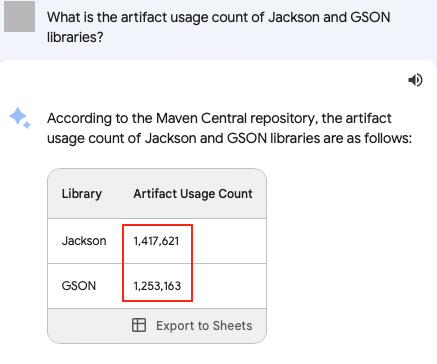
\includegraphics[scale=.45]{images/BARD-donwload-count-1.png}
        \caption{Response from BARD}
    \label{fig:bard-download}
    \end{subfigure}
    \begin{subfigure}{.48\textwidth}
    \centering
        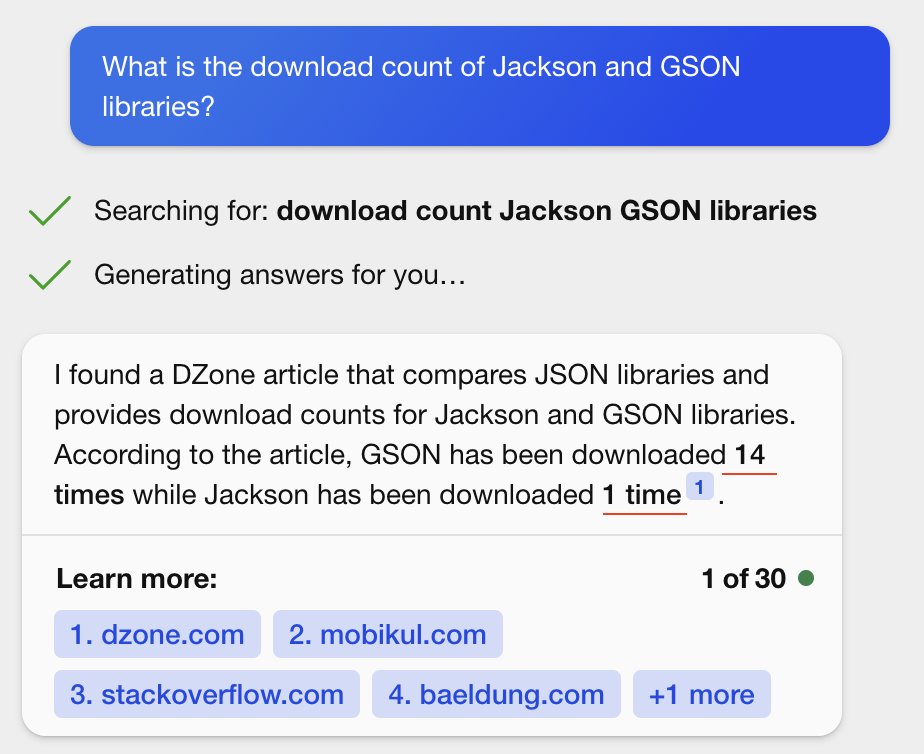
\includegraphics[scale=.45]{images/BING-download-count.png}
        \caption{Response from BING Chat}
    \label{fig:chatgpt-download}
    \end{subfigure}
    \caption{Stark contrast in response from BARD and ChatGPT for the usage count of Jackson and GSON libraries. According to BARD, both of these libraries have been used for more than 1 million times and according to BING chat these libraries are downloaded less than 100 times.}
    \label{fig:chatbot-comparison-download}
\end{figure*}

The small experiments raised concern about the reliability of the responses of the chatbots for the library comparison analysis. We were then curious if the industry practitioners also find similar reliability concerns and how they are considering using chatbots for the library selection process.


\subsubsection{Evaluation on the Usage of ChatGPT and BARD for Library Selection}
We conducted a survey to collect insights regarding chatbot usage among the interviewees. 20 out of 24 interviewees responded to our anonymous online survey.

\textbf{Survey Settings.} In the survey, we asked whether the practitioners already considered using ChatGPT/BARD and what advantages and disadvantages they consider for using those. Since BARD is available only in limited countries, we created the prompt and response example using only ChatGPT so that respondents can recognize familiar tools easily. Also, since we already experimented with Jackson and GSON libraries, we queried about libraries from a different domain (natural language processing - NLP) in the survey.

We asked the following questions in the survey while providing the ChatGPT screenshots when applicable:
\begin{enumerate}
    \item \textbf{Reliability on ChatGPT Response.} We asked participants how much they would rely on the response of ChatGPT against the prompt \textit{"What is a good library in Python for NLP?"}.
    \item \textbf{Next Action after ChatGPT Response.} We then asked an explanatory prompt to ChatGPT \textit{"How easy it is to use Spacy?"}, and asked the participants what would be their next action plan - whether they will trust the response to install the library instantly or will further inquire inside or outside ChatGPT.
    \item \textbf{Comparing Data Interpretation between ChatGPT and Human.} Since ChatGPT is based on a language sequence model that can predict the next token and is trained on undisclosed online data, it was interesting to see how it responds when we give specific library reviews extracted from Stack Overflow. So, with a given review data, we prompted ChatGPT \textit{"How easy it is to use the library strictly based on the given conversation?"}. Then we asked the survey participant whether they agree with the response ChatGPT provided or not.
\end{enumerate}
After the above specific ChatGPT scenarios, we asked the participants their opinion about the quality and reliability concerns of ChatGPT along with their recommendations for future improvement.

\textbf{Survey Findings.}
\begin{enumerate}
    \item \textbf{Usage of ChatGPT.} 
    50\% of respondents said they did not consider using ChatGPT for library selection. The primary reasons they did not consider ChatGPT were lack of reliable research on ChatGPT response, lack of reference for the response, and lack of credibility of the response: \quotebox{}{I have not started using it yet. Chatbots like ChatGPT summarize the comparisons quite well. But they do not always include references and hence credibility needs to be cross-checked almost always.}
    Only 15\% responded that they started using ChatGPT. They considered ChatGPT as an initial high-level information source and they also shared the quality concerns: \quotebox{}{Yes, I have considered chatbots to select and compare libraries. It gives me an initial idea about different libraries quickly without checking search engine results.}
    The rest of the participants did not explicitly mention whether they are using it or not. 
    \item \textbf{Reliability on ChatGPT Response.} 
    No participant said that they would fully rely on the response.
    60\% participants considered asking ChatGPT further about the recommended library and 35\% considered asking about alternative libraries.
    20\% participants would not even trust this recommendation as the source of ChatGPT's response was unknown.
    \item \textbf{Next Action after ChatGPT Response.} 
    85\% participants preferred searching online (using search engines) about spaCy (the library that ChatGPT suggested for NLP) and its alternative libraries listed by ChatGPT.
    60\% responded that they would go to the official documentation of the library after the initial ChatGPT response 
    55\% participants would go online and search Stack Overflow or similar sites to learn about other developers' opinions.
    55\% participants would choose to ask ChatGPT again to provide API samples. 25\% would have doubt about the opinion of ChatGPT and would ask it further elaborative questions.
    
    \item \textbf{Comparing Data Interpretation between ChatGPT and Human.}
    We got mixed results from participants on whether they agreed with the ChatGPT response when a specific library-related conversation was provided. 50\% respondents disagreed with ChatGPT's answer, 20\% agreed and the remaining 30\% were not sure about the correctness of the response provided by ChatGPT.

    \item \textbf{Recommendations for Library Selection}
    The majority of the respondents (85\%) suggested providing additional references to online data sources to support the response of ChatGPT. 20\% participants opined that further challenging questions could be asked to ChatGPT. Some of them also recommended developing a domain-specific chatbot tuned specifically for reusable libraries that can provide better answers compared to general-purpose chatbots.
\end{enumerate}

 In general, the majority of participants shared strong opinions against the reliability, consistency, and validity of ChatGPT responses. They could consider it as an initial discovery source but would not make the final decision based on it. One participant summed it this way: 
 %\ab{Quote this the same way you quote interviews}
 \quotebox{}{I never trust anything chatbot returns, but it's still helpful for research. It's helpful to treat it as the smart, loud, slightly drunk guy at the party. You may gain some great info, but you really don't trust anything he says.}

 
\subsection{Tool Agnostic Relative Priorities of Library Selection Factors}
Because of the reliability concerns of ChatGPT and BARD in library comparison tasks, future researchers might need to develop some comparison tools based on large-scale data mining techniques to calculate the aspect-specific scores as outlined in section \ref{sec:mock-up} or will need to refine the response of those chatbots. However, we found from the industry evaluation that practitioners would always need to use variable priorities depending on their conditions. Interviewees also suggested providing some default priorities to help developers update according to their needs. Hence,
it would be a great convenience if we can provide a default factor-wise priority or weight score in the comparison tool.

%During our interviews while we discussed about library selection factors, we often asked developers whether they treat all the factors equally important. All participants unanimously expressed that all the factors have different priorities to them in general. That was also one motivation to provide weight of the factors in the comparison tool described in previous section. Though we explained in detail that guiding principles influence the library selection factors to great deal, we realized that a generic priority of library selection criteria would be helpful for developers' common understanding and for implementation of any comparative analysis tool.

% Table generated by Excel2LaTeX from sheet 'Priority of factors'
\begin{table}[htbp]
  \centering
  \caption{Relative priorities of library selection factors. The higher score reflects higher priority practitioners put on when selecting a third party library. The priority score is normalized out of 10. Our recommended cut-off factors are marked with asterisk (*).}
    \begin{tabular}{llr}
    \toprule
    \textbf{Factor} & \textbf{Category} & \multicolumn{1}{l}{\textbf{Priority}} \\
    \midrule
    Performance & Software &                 8.2  \\
    Stability & Software &                 7.8  \\
    Licence* & Commercial &                 7.5  \\
    Documentation & Commercial &                 7.3  \\
    Security* & Software &                 6.9  \\
    Compatibility* & Software &                 6.4  \\
    Active Development & Maintenance &                 6.2  \\
    Popularity & External &                 6.0  \\
    Supported by Own Organization & Maintenance &                 5.9  \\
    Ease of Use & Software &                 5.5  \\
    Capability of Library* & Software &                 5.5  \\
    Dependency & Commercial &                 5.4  \\
    Flexibility & Software &                 5.4  \\
    Open Source Software & Commercial &                 5.2  \\
    Community Support & Maintenance &                 5.2  \\
    Cost  & Commercial &                 5.1  \\
    Used by Reputed Companies & Maintenance &                 4.9  \\
    Availability of Demo & Commercial &                 4.8  \\
    Large Community & Maintenance &                 4.5  \\
    Supported by Reputed Organization & Maintenance &                 4.4  \\
    Customer Support & Maintenance &                 4.4  \\
    Familiarity & External &                 4.3  \\
    Size of Library & Software &                 4.2  \\
    Search Engine Ranking & External &                 4.1  \\
    Ease of Installation & Software &                 3.6  \\
    Interesting Interface & Software &                 2.7  \\
    Detailed Benchmark & External &                 2.6  \\
    Roadmap & Commercial &                 2.4  \\
    \bottomrule
    \end{tabular}%
  \label{tab:factor-priority}%
\end{table}%

In this regard, during the member checking survey (described in the quality evaluation section), we also asked our interview participants how they compare among all the 28 library selection factors. For each factor, we let them choose a score on a sliding scale of 20. We used the ``Statement randomization'' feature of Qualtrics\footnote{\url{https://www.qualtrics.com}} software to randomize the list of the selection factors to avoid response order bias \cite{israel1990can}.

%\ab{Why do you have these blue?}
\td{11} out of \td{13} respondents of the survey provided their scoring of relative priorities of library selection criteria. Table \ref{tab:factor-priority} shows the average priority of selection factors normalized on a scale of 10. Participants chose \code{performance}, \code{stability}, \code{license}, \code{documentation}, and \code{security} as their top priority factors. Though we observed that the {\principle} can significantly influence the priority of these factors, we recommend \code{security} and \code{license} to be `cut-off' factors for any team so that they do not compromise with non-supported license and security vulnerabilities. We observed that two other factors \code{capability of library} and \code{compatibility} are also cut-off factors in the sense that if a library is not compatible with the target environment and does not perform the intended task, there is no point in using such a library. We marked these four factors with an asterisk to denote them as cut-off factors in Table \ref{tab:factor-priority}. We believe any future research could enhance this generic priority of factors to a more customized priority score followed by the {\principle} to respect the conditions of particular organizations and development teams.